\documentclass{article}
\usepackage{makeidx}
\usepackage{hyperref}
\usepackage{amsmath}
\usepackage{amssymb}
\usepackage{xcolor}
\usepackage{graphicx}

\title{Deep Learning Notes}
\author{Haotian Chen}
\date{}

\makeatletter
\renewcommand\paragraph{\@startsection{paragraph}{4}{\z@}%
                                     {-3.25ex\@plus -1ex \@minus -.2ex}%
                                     {1.5ex \@plus .2ex}%
                                     {\normalfont\normalsize\bfseries}}
\makeatletter

\hypersetup{
    colorlinks=true,
    linkcolor=blue,
    urlcolor=cyan,
}

\setcounter{tocdepth}{4}
\setcounter{secnumdepth}{4}

\makeindex



\begin{document}

\maketitle

\clearpage

\tableofcontents{}

\clearpage

\section{Neural Networks and Deep Learning}

\subsection{Binary Classification}

Use logistic regression to build a binary classifier.

\begin{center}
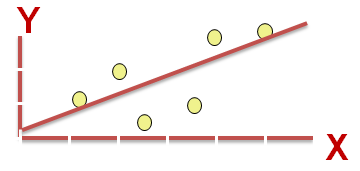
\includegraphics[scale=0.4]{./images/binary_classification.png}
\end{center}

\noindent \textbf{training data}:
\[(x^{(i)}, y^{(i)})\:for\:i = 1, \dots, m\]

\[
x^{(i)} = 
\begin{bmatrix}
x^{(i)}_1\\
x^{(i)}_2\\
\vdots\\
x^{(i)}_n
\end{bmatrix}
,
y^{(i)} = y^{(i)}_1
\]

\[X =
\begin{bmatrix}
x^{(1)} & x^{(2)} & \dots & x^{(m)}
\end{bmatrix}
,
Y =
\begin{bmatrix}
y^{(1)} & y^{(2)} & \dots & y^{(m)}
\end{bmatrix}
\]

\subsection{Logistic Regression}

\noindent Logistic regression is a statistical model that uses a logistic function to model a binary dependent variable.

\bigskip

\noindent Given \(x\), want \(\hat{y} = P(y = 1 | x)\), where \(0 \leq \hat{y} \leq 1\), \(x \in \mathbb{R}^{n_x}\), \(w \in \mathbb{R}^{n_x}\), \(b \in \mathbb{R}\)

\[z = w^Tx + b\]
\[\hat{y} = \sigma(z)\]

\printindex

\end{document}